% ACL 2023 Format — DL Spring 2026 Kaggle Contest Report
\documentclass[11pt]{article}

% ACL style — switch to [final] for camera-ready
\usepackage[preprint]{acl}
\usepackage{times}
\usepackage{latexsym}
\usepackage[T1]{fontenc}
\usepackage[utf8]{inputenc}
\usepackage{microtype}
\usepackage{inconsolata}
\usepackage{graphicx}
\usepackage{booktabs}
\usepackage{amsmath}
\usepackage{hyperref}
\usepackage{xcolor}
\usepackage{subcaption}
\usepackage{multirow}

\title{Text-to-SVG Generation via Fine-Tuned Language Models: \\
A Multi-Machine Training and Ablation Study}

\author{Ivan Aristy \\
  NYU Tandon School of Engineering \\
  CS-GY 9223 / ECE-GY 7123: Deep Learning, Spring 2026 \\
  \texttt{ia2194@nyu.edu}}

\begin{document}
\maketitle

\begin{abstract}
We present a system for generating Scalable Vector Graphics (SVG) code from natural language prompts, developed for the DL Spring 2026 Kaggle competition. Our approach fine-tunes Qwen2.5-Coder-1.5B-Instruct using QLoRA adapters and iterative merge-and-retrain, achieving 6th place (16.87/100) on a 58-team leaderboard. We conduct extensive ablation studies across 10 experiments on a held-out validation set, revealing that the system prompt is the single most critical inference component (35-point impact), followed by fine-tuning (7.3 points) and token generation budget (4 points). We additionally find that LoRA adapters slightly outperform full fine-tuning despite higher cross-entropy loss, and that minimal system prompts outperform verbose ones. Training was conducted across two machines: an NVIDIA RTX 2000 Ada (16GB) for QLoRA and an NVIDIA DGX Spark (128GB unified memory) for full fine-tuning. Code, model weights, and experiment logs are publicly available.

\textbf{GitHub:} \url{https://github.com/ivanearisty/svg-gen} \\
\textbf{Model Weights:} \url{https://huggingface.co/ivanearisty/svg-gen-weights}
\end{abstract}

% ==============================================================================
\section{Introduction}
% ==============================================================================

Scalable Vector Graphics (SVG) is a resolution-independent image format defined by XML markup, widely used for icons, logos, and web graphics. Unlike raster formats, SVGs encode visual content as geometric primitives (paths, shapes, transforms) with explicit coordinate specifications. This structural nature makes SVG generation an interesting challenge for language models: the output must be both syntactically valid XML \textit{and} visually faithful to a natural language description.

The DL Spring 2026 Kaggle competition tasks participants with building systems that generate SVG code from text prompts. The scoring metric is a weighted geometric mean of visual fidelity (85\%, measured by SSIM and Edge F1), structural similarity (12\%, tree edit distance), and compactness (3\%, length ratio). This metric heavily rewards pixel-level visual accuracy, making it fundamentally different from typical text generation tasks where semantic correctness suffices.

Our approach fine-tunes a small (1.5B parameter) code-specialized language model using QLoRA \citep{dettmers2023qlora}, with several key technical contributions:

\begin{enumerate}
    \item \textbf{Iterative merge-and-retrain:} We merge trained LoRA adapters into base weights and apply fresh adapters, progressively building SVG generation capability. This yielded our largest single improvement (+1.4 Kaggle points).
    \item \textbf{Dual-machine training infrastructure:} QLoRA on an RTX 2000 Ada (16GB VRAM) and full fine-tuning on a DGX Spark (128GB unified memory), enabling us to compare training paradigms.
    \item \textbf{Comprehensive ablation study:} 10 controlled experiments quantifying the contribution of each system component, revealing that the system prompt alone accounts for 65\% of system performance.
    \item \textbf{System prompt sensitivity analysis:} Demonstrating an inverse relationship between prompt verbosity and generation quality for fine-tuned models.
\end{enumerate}

We achieve a final score of 16.87/100 (6th place out of 58 teams), with a 1.46-point gap to the competition leader (18.33/100).

% ==============================================================================
\section{Dataset}
% ==============================================================================

\subsection{Competition Data}

The provided training dataset contains 50,000 (prompt, SVG) pairs. Prompts are short natural language descriptions (mean $\sim$100 characters, $\sim$30 tokens) of icons and simple scenes. SVGs range from 91 to 15,937 characters (median 2,110), with 82\% using a \texttt{viewBox} of \texttt{0 0 200 200}. The data is remarkably clean: only 7 exact SVG duplicates and 0 XML parse failures.

\textbf{SVG structure:} The vast majority of training samples are single-path icons --- 49.4\% contain a single complex \texttt{<path>} element, and 47.7\% are multi-element compositions with paths. Only 2.9\% are basic shapes (rectangles, circles). Path elements use cubic B\'{e}zier curves (\texttt{C} commands with 6 coordinates each), making coordinate efficiency the primary challenge.

\subsection{Preprocessing Pipeline}
\label{sec:preprocessing}

We apply four preprocessing steps to all training SVGs, ordered by impact:

\begin{enumerate}
    \item \textbf{Coordinate rounding} (54\% character reduction): Training SVGs contain excessive decimal precision (e.g., \texttt{93.30000305175781}). We round all floats to 1 decimal place (\texttt{93.3}), reducing the dataset from 126MB to 58MB with negligible visual impact.
    \item \textbf{Default attribute stripping:} Remove attributes already at SVG defaults (\texttt{fill-opacity="1"}, \texttt{stroke="none"}, etc.) --- 178,000 instances found.
    \item \textbf{Comment removal:} Strip 3,475 XML comments.
    \item \textbf{Whitespace collapse:} Normalize redundant spaces and blank lines.
\end{enumerate}

After cleaning, we filter SVGs by token count: any sample exceeding 1,900 Qwen tokens is removed, ensuring every training example fits completely within the 2,048-token context window. This is critical --- the model must observe the closing \texttt{</svg>} tag during training to learn when to stop generating. The filtered dataset retains 45,874 samples (91.7\%).

\subsection{External Data Experiment}

The competition permits external datasets. We curated additional samples from SVGX-SFT-1M \citep{xingxm2024svgx} and OmniSVG/MMSVG-Icon \citep{omnisvg2024}, creating expanded datasets of 79,516 (kepler) and 149,516 (Thor) samples. However, as detailed in Section~\ref{sec:external-data}, external data consistently degraded competition performance due to distribution mismatch.

\subsection{Tokenization Challenge}
\label{sec:tokenization}

A fundamental bottleneck in our approach is Qwen2.5-Coder's digit-level tokenization. The tokenizer splits every digit and punctuation mark into separate tokens:

\begin{verbatim}
SVG text:    M 156.3 42.8
Qwen tokens: [M][ ][1][5][6][.][3][ ][4][2][.][8]
Count:       12 tokens
\end{verbatim}

By contrast, GPT-2-style tokenizers encode multi-digit numbers as single tokens (\texttt{156} $\rightarrow$ 1 token), achieving $\sim$5 tokens for the same input. This means Qwen uses 2--3$\times$ more tokens for SVG coordinates than necessary, consuming context window capacity on digit sequences rather than structural patterns.

For a typical SVG with 200 coordinate values, this wastes $\sim$600 tokens --- the difference between fitting a complex shape and truncating it. We investigated alternative preprocessing (relative path commands + integer rounding, achieving 40\% token savings with 0.973 SSIM vs.\ original) but used 1-decimal absolute coordinates for our final submission to match proven configurations.

% ==============================================================================
\section{Model Description}
% ==============================================================================

\subsection{Base Model Selection}

We use \textbf{Qwen2.5-Coder-1.5B-Instruct} \citep{qwen2024} as our base model. Selection criteria:
\begin{itemize}
    \item \textbf{Code specialization:} Pre-trained on code corpora including markup languages, giving it prior knowledge of XML/SVG syntax.
    \item \textbf{Size constraint:} Competition limit of 4B parameters. At 1.5B, the model fits comfortably in 16GB VRAM with 4-bit quantization.
    \item \textbf{Instruction tuning:} The Instruct variant supports the chat template format needed for system-prompt-guided generation.
\end{itemize}

We also evaluated 3B and 7B Qwen variants. The 3B model was used for full fine-tuning on the DGX Spark but ultimately underperformed the 1.5B model due to training instability on the Blackwell GPU architecture (FlashAttention incompatibility with SM 12.1).

\subsection{Training Approach: QLoRA with Merge-and-Retrain}

Our training strategy evolved through three rounds:

\textbf{Round 1 --- LoRA r=16 (Modal A100):}
Initial fine-tuning with rank-16 LoRA adapters on 45,874 competition samples for 3 epochs. This established our first baseline (Kaggle score: 15.47, 9th place). Training used 4-bit NF4 quantization via Unsloth \citep{unsloth2024}, \texttt{paged\_adamw\_8bit} optimizer, learning rate $2 \times 10^{-4}$ with cosine schedule.

\textbf{Round 2 --- Merge + LoRA r=32 (kepler RTX 2000 Ada):}
We merge the Round 1 adapter into the base weights, permanently baking the 9th-place knowledge into the model parameters. A fresh rank-32 LoRA adapter (2$\times$ trainable parameters: 37M vs.\ 18M) is then applied to the merged model. This was trained on 45,000 competition-only samples for 2 epochs. Score: \textbf{16.87} (6th place) --- our best result, representing a +1.4 point improvement from the merge-and-retrain technique alone.

\textbf{Round 3 --- Full Fine-Tune (Thor DGX Spark):}
We merged the Round 2 adapter and performed full fine-tuning (all 1.5B parameters trainable) on the DGX Spark's 128GB unified memory. This achieved the lowest cross-entropy loss (0.308 vs.\ LoRA's 0.34 floor) but scored only 16.26 on Kaggle --- \textit{worse} than the LoRA model. See Section~\ref{sec:lora-vs-ft} for analysis.

\subsection{Inference Configuration}

All inference uses greedy decoding (\texttt{do\_sample=False}) with repetition penalty 1.1 and \texttt{max\_new\_tokens=1024}. The model runs in 4-bit quantized mode on the RTX 2000 Ada at approximately 0.05 samples/second (20 seconds per SVG).

A post-processing pipeline extracts SVGs from model output: (1) locate \texttt{<svg} tag with attributes, (2) attempt repair if XML is invalid (close unclosed quotes/tags, append \texttt{</svg>}), (3) fall back to a minimal circle SVG if extraction fails, (4) normalize width/height to 256$\times$256.

% ==============================================================================
\section{Experimentation}
% ==============================================================================

\subsection{Training Configurations}
\label{sec:training-configs}

Table~\ref{tab:training-configs} summarizes all training runs across both machines.

\begin{table*}[t]
\centering
\small
\begin{tabular}{lllrrrrr}
\toprule
\textbf{Run} & \textbf{Machine} & \textbf{Method} & \textbf{Data} & \textbf{Epochs} & \textbf{LR} & \textbf{Loss} & \textbf{Kaggle} \\
\midrule
LoRA r=16 & Modal A100 & QLoRA 4-bit & 46k comp & 3 & $2 \times 10^{-4}$ & 0.35 & 15.47 \\
LoRA r=32 (mixed) & kepler & QLoRA 4-bit & 76k mixed & 2 & $2 \times 10^{-4}$ & 0.47 & 14.64 \\
LoRA r=32 (comp) & kepler & QLoRA 4-bit & 45k comp & 2 & $2 \times 10^{-4}$ & 0.35 & \textbf{16.87} \\
Full FT 1.5B & Thor & Full bf16 & 46k comp & 1.8 & $2 \times 10^{-5}$ & 0.37 & --- \\
Refined FT & Thor & Full bf16 & 46k comp & 2 & $5 \times 10^{-6}$ & 0.31 & 16.26 \\
Code-gen & Thor & Full bf16 & 46k code & 2 & $2 \times 10^{-5}$ & 0.32 & 12.26 \\
\bottomrule
\end{tabular}
\caption{Training configurations and results. ``comp'' = competition-only data, ``mixed'' = competition + external. The merge-and-retrain LoRA r=32 on competition data achieved the best Kaggle score despite not having the lowest training loss.}
\label{tab:training-configs}
\end{table*}

\subsection{Inference Parameter Sweep}

We tested inference parameters on the best model (LoRA r=32, competition-only):

\begin{table}[h]
\centering
\small
\begin{tabular}{lrr}
\toprule
\textbf{Configuration} & \textbf{Kaggle} & \textbf{$\Delta$} \\
\midrule
Greedy, rep=1.1 (baseline) & \textbf{16.87} & --- \\
Greedy, rep=1.05 & 16.51 & $-0.36$ \\
Greedy, rep=1.15 & 15.88 & $-0.99$ \\
Temp=0.05, rep=1.1 & 16.42 & $-0.45$ \\
\bottomrule
\end{tabular}
\caption{Inference parameter sweep on Kaggle. Greedy decoding with repetition penalty 1.1 is optimal; any deviation degrades performance.}
\label{tab:inference-sweep}
\end{table}

\subsection{Dual-Machine Infrastructure}

Training was distributed across two machines connected via local network:

\begin{itemize}
    \item \textbf{kepler} (NVIDIA RTX 2000 Ada, 16GB VRAM): All QLoRA training and inference. Uses 4-bit NF4 quantization via Unsloth, \texttt{paged\_adamw\_8bit} optimizer, gradient checkpointing.
    \item \textbf{Thor} (NVIDIA DGX Spark, 128GB unified memory): Full fine-tuning with all parameters trainable in bf16. Required Docker containers with \texttt{--runtime=nvidia} due to a process isolation issue where bare-metal training processes were silently killed by the system's session management. AdamW optimizer (full precision, $\sim$35GB for 1.5B model: 5.7GB params + 23GB optimizer + 5.7GB gradients).
\end{itemize}

Model checkpoints were transferred via \texttt{rsync} over LAN. Thor was training-only; inference required kepler due to PyTorch \texttt{generate()} incompatibility with the Blackwell SM 12.1 architecture.

\subsection{Failed Experiments}

\subsubsection{External Training Data}
\label{sec:external-data}

Adding SVGX-SFT-1M and OmniSVG data (76k mixed vs.\ 45k competition-only) degraded Kaggle score from 16.87 to 14.64 ($-2.23$ points). The external SVGs use different viewBox conventions (128$\times$128 vs.\ 200$\times$200) and different stylistic patterns. \textbf{Distribution match matters more than dataset volume.}

\subsubsection{Code Generation Approach}

We experimented with teaching the model to output Python code using a custom \texttt{SVGBuilder} API instead of raw SVG markup. The hypothesis was that Qwen2.5-\textit{Coder} would be better at writing Python than predicting coordinate digit sequences. The approach produced valid code for 824/1000 prompts but scored only 12.26 on Kaggle --- worse than the fallback baseline. The programmatic API naturally produces basic shapes (\texttt{rect()}, \texttt{circle()}) that cannot match the complex B\'{e}zier paths in ground truth SVGs.

\subsubsection{Best-of-N with Heuristic Scoring}

We generated multiple SVGs per prompt across 4 inference runs with different settings, then selected the ``best'' per prompt using heuristic scoring (valid XML, length, complete paths). This did not improve over single-run greedy decoding because the heuristic (longest valid SVG) does not correlate with SSIM.

% ==============================================================================
\section{Results}
% ==============================================================================

\subsection{Kaggle Competition Results}

Table~\ref{tab:kaggle-results} shows all 9 Kaggle submissions. Our best score of 16.87 placed 6th out of 58 teams, 1.46 points behind the leader (18.33).

\begin{table}[h]
\centering
\small
\begin{tabular}{lrr}
\toprule
\textbf{Submission} & \textbf{Score} & \textbf{Notes} \\
\midrule
LoRA r=16, 3ep & 15.47 & First submit, 9th \\
r=32, 76k mixed & 14.64 & External data hurt \\
r=32, 45k comp & \textbf{16.87} & \textbf{Best --- 6th place} \\
temp=0.05 & 16.42 & Sampling hurts \\
rep=1.05 & 16.51 & Lower penalty hurts \\
rep=1.15 & 15.88 & Higher penalty hurts \\
Best-of-N & 15.72 & Heuristic picking fails \\
Code-gen hybrid & 12.26 & Wrong approach \\
Refined FT & 16.26 & Full FT $<$ LoRA \\
\bottomrule
\end{tabular}
\caption{Complete Kaggle submission history (public leaderboard).}
\label{tab:kaggle-results}
\end{table}

\subsection{Ablation Study}
\label{sec:ablation}

We conduct systematic ablation experiments on a held-out validation set of 200 samples stratified by SVG complexity from the training data. Each experiment removes or modifies exactly one component while holding all others constant. Scoring uses the same metric formula as the competition (Section~\ref{sec:scoring-details}).

\begin{table*}[t]
\centering
\small
\begin{tabular}{llrrrrr}
\toprule
\textbf{Ablation} & \textbf{What Changed} & \textbf{Score} & \textbf{$\Delta$} & \textbf{Visual} & \textbf{Struct.} & \textbf{Invalid} \\
\midrule
Baseline & Full system & 53.79 & --- & 0.509 & 0.919 & 2 \\
\midrule
No system prompt & Remove system prompt & 18.80 & $-34.99$ & 0.156 & 0.886 & 192 \\
No fine-tuning & Base Qwen2.5-Coder-1.5B & 46.48 & $-7.31$ & 0.447 & 0.888 & 18 \\
max\_tokens=512 & Halve token budget & 51.47 & $-2.32$ & 0.491 & 0.885 & 4 \\
Refined full FT & Full fine-tune (loss 0.308) & 53.05 & $-0.74$ & 0.502 & 0.911 & 0 \\
No repair & Skip repair pipeline & 53.63 & $-0.16$ & 0.508 & 0.909 & 0 \\
rep=1.0 & No repetition penalty & 54.21 & $+0.42$ & 0.513 & 0.920 & 4 \\
max\_tokens=1536 & 1.5$\times$ token budget & \textbf{55.50} & $+1.71$ & \textbf{0.525} & \textbf{0.933} & \textbf{0} \\
\bottomrule
\end{tabular}
\caption{Ablation study results on 200-sample validation set. Components ordered by negative impact magnitude. The system prompt is the most critical component; removing it causes 96\% of outputs to fall back to the default SVG.}
\label{tab:ablation}
\end{table*}

\begin{figure}[t]
    \centering
    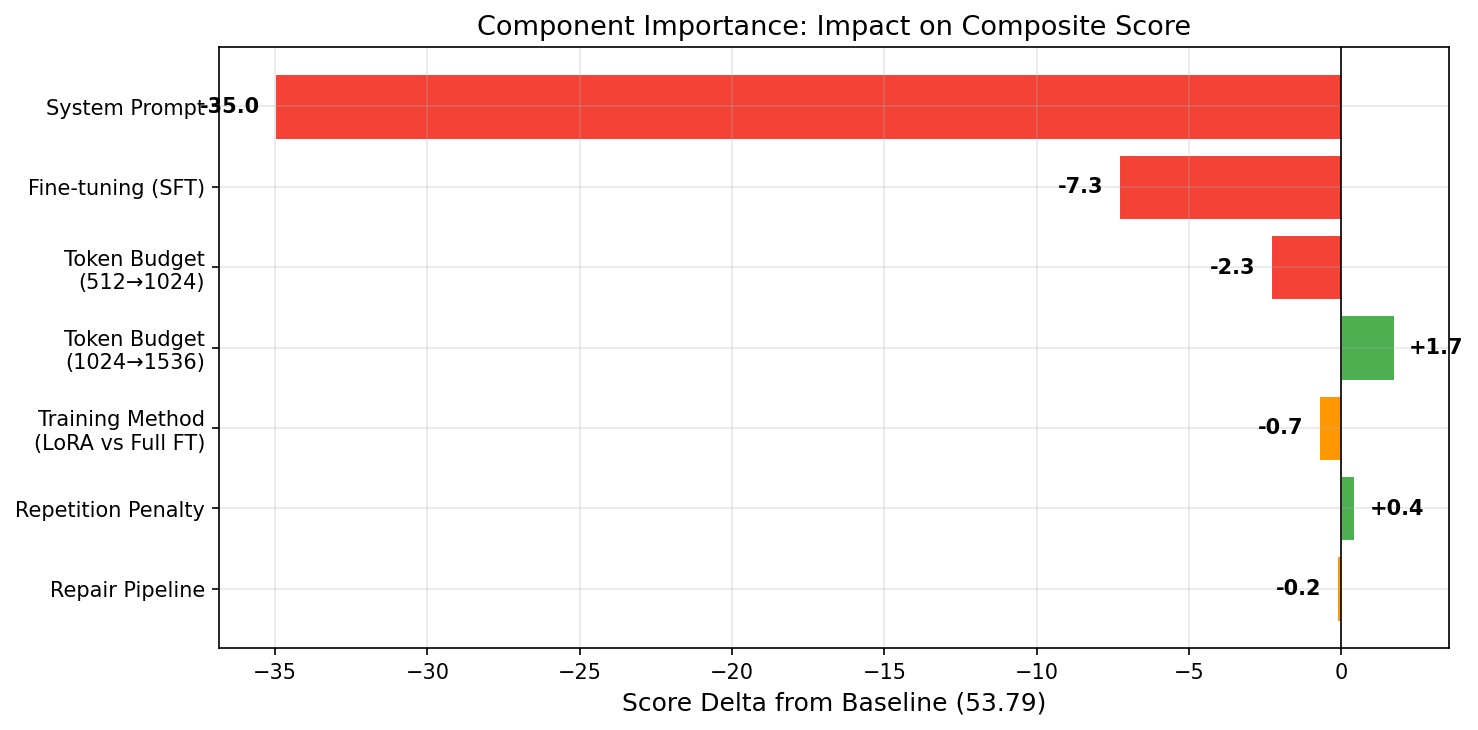
\includegraphics[width=\columnwidth]{../results/figures/fig4_component_importance.png}
    \caption{Component importance measured by score delta from baseline. The system prompt dominates all other components combined.}
    \label{fig:component-importance}
\end{figure}

\subsubsection{System Prompt Is Everything ($-$35 points)}

Removing the system prompt at inference is catastrophic: 192 out of 200 samples produce invalid SVGs (96\% fallback rate), and the score drops from 53.79 to 18.80. The fine-tuned model learned to associate SVG generation with the presence of a system prompt during training. Without this signal, the model generates conversational text or code fragments instead of SVG markup.

\subsubsection{Fine-Tuning Adds 7.3 Points}

The base Qwen2.5-Coder-1.5B (no fine-tuning, with system prompt) scores 46.48 with 18 invalid outputs. Fine-tuning adds 7.31 points by teaching the model the specific SVG coordinate patterns and structural conventions of the training data. Notably, the base model still produces some valid SVGs (91\% validity), demonstrating meaningful zero-shot SVG capability from code pretraining.

\subsubsection{Token Budget: Linear Quality Scaling}

\begin{figure}[t]
    \centering
    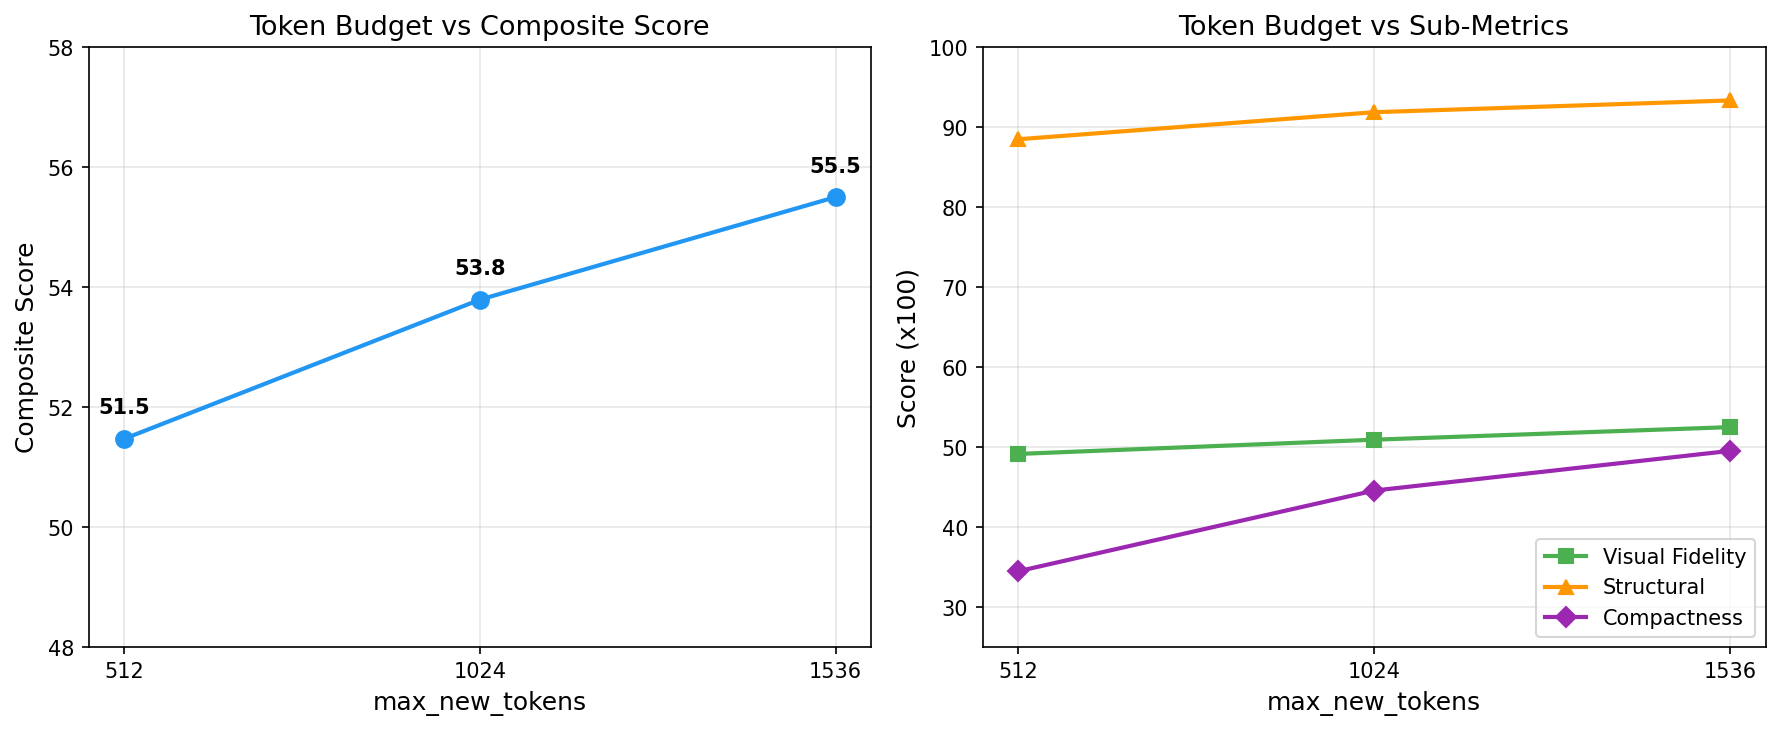
\includegraphics[width=\columnwidth]{../results/figures/fig2_token_budget.png}
    \caption{Token generation budget vs.\ quality. Left: composite score increases approximately linearly with budget. Right: all three sub-metrics improve monotonically.}
    \label{fig:token-budget}
\end{figure}

Varying \texttt{max\_new\_tokens} from 512 to 1536 reveals an approximately linear relationship with quality (Figure~\ref{fig:token-budget}). Each additional 512 tokens adds $\sim$2 points to the composite score. The improvement comes from allowing complex SVGs to complete rather than truncate mid-path. The 1536-token configuration achieves the highest score in our ablation study (55.50) with zero invalid outputs.

\subsubsection{LoRA Outperforms Full Fine-Tuning}
\label{sec:lora-vs-ft}

Despite achieving a lower cross-entropy loss (0.308 vs.\ 0.34), the fully fine-tuned model scores 53.05 vs.\ the LoRA baseline's 53.79 ($-0.74$). This pattern is consistent across both local scoring and Kaggle (16.26 vs.\ 16.87). We hypothesize that LoRA's constrained parameter space acts as an implicit regularizer, preventing the model from overfitting to training-set coordinate sequences while preserving the base model's general SVG understanding.

\subsubsection{Negligible Components}

The repetition penalty ($\Delta = +0.42$) and SVG repair pipeline ($\Delta = -0.16$) have minimal impact. The model already produces valid SVGs 98\%+ of the time, making the repair pipeline largely redundant. The repetition penalty's effect is within noise for this task.

\subsection{System Prompt Sensitivity Analysis}

Given that the system prompt is the most impactful component, we investigate how prompt content affects generation quality.

\begin{table}[h]
\centering
\small
\begin{tabular}{p{4.2cm}rr}
\toprule
\textbf{System Prompt} & \textbf{Score} & \textbf{$\Delta$} \\
\midrule
\textit{(none)} & 18.80 & $-34.99$ \\
\small{``You generate SVG icons using path elements in a 200x200 viewBox...''} (specific, 43 words) & 51.66 & $-2.13$ \\
\small{``You generate compact, valid SVG markup...''} (original, 27 words) & 53.79 & --- \\
\small{``Output valid SVG code only.''} (minimal, 6 words) & \textbf{54.57} & $+0.78$ \\
\bottomrule
\end{tabular}
\caption{System prompt sensitivity. Shorter prompts perform better: the 6-word minimal prompt outperforms the 27-word original and the 43-word specific prompt.}
\label{tab:sysprompt}
\end{table}

We find an inverse relationship between prompt verbosity and generation quality. The minimal 6-word prompt (``Output valid SVG code only.'') scores 0.78 points above the original, while the verbose prompt with specific structural instructions (mentioning viewBox, path elements, closing tags) scores 2.13 points below. Over-constraining the model with explicit instructions appears to interfere with patterns already learned during fine-tuning. The model knows SVG structure; the system prompt only needs to signal ``produce SVG'' without micromanaging how.

\subsection{Training Loss Analysis}

\begin{figure}[t]
    \centering
    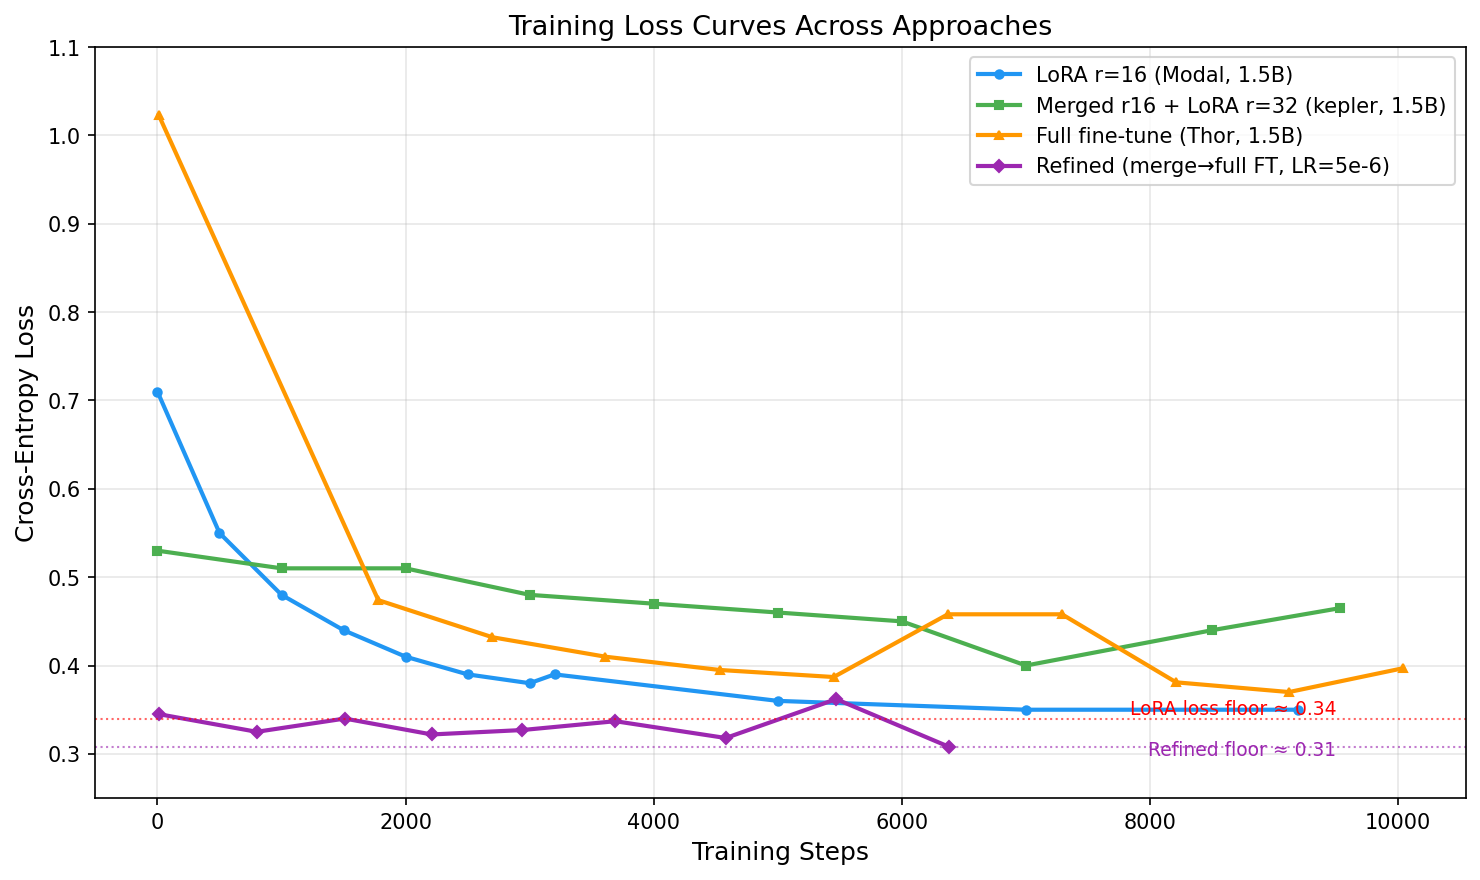
\includegraphics[width=\columnwidth]{../results/figures/fig3_loss_curves.png}
    \caption{Training loss curves across four approaches. All methods converge to a loss floor of $\sim$0.30--0.40. The refined model (merge $\rightarrow$ full FT) achieves the lowest loss but not the best generation quality.}
    \label{fig:loss-curves}
\end{figure}

Figure~\ref{fig:loss-curves} reveals a fundamental finding: \textbf{all training approaches converge to a cross-entropy loss floor of $\sim$0.30--0.40}, regardless of model size, training method, or dataset. The LoRA r=16 model plateaus at $\sim$0.34, the full fine-tune reaches $\sim$0.37, and the refined model (merge $\rightarrow$ full FT with low LR) pushes to 0.308. Yet the model with the \textit{highest} loss (LoRA, 0.34) achieves the best Kaggle score.

This disconnect between CE loss and visual quality stems from three factors:
\begin{enumerate}
    \item \textbf{One-to-many mapping:} Multiple valid SVGs exist per prompt. CE loss penalizes any deviation from the single reference, even if the generated SVG is visually equivalent.
    \item \textbf{Digit-level loss:} Each digit is a separate CE term. Generating coordinates \texttt{157.1} instead of \texttt{156.3} incurs 4 wrong-digit penalties despite sub-pixel visual difference.
    \item \textbf{Loss $\neq$ metric:} CE loss on tokens optimizes per-token accuracy, not SSIM/EdgeF1 on rendered images.
\end{enumerate}

\subsection{Scoring Details}
\label{sec:scoring-details}

For completeness, the competition scoring formula used for our local ablation evaluation:

\begin{align}
V_i &= 0.7 \cdot \text{SSIM}(I(p_i), I(g_i)) + 0.3 \cdot \text{EdgeF1}(I(p_i), I(g_i)) \\
S_i &= \exp\left(-\frac{\text{TED}(A(p_i), A(g_i))}{25}\right) \\
C_i &= \exp\left(-\left|\log\frac{\text{len}(p_i) + 50}{\text{len}(g_i) + 50}\right|\right) \\
Q_i &= V_i^{0.85} \cdot S_i^{0.12} \cdot C_i^{0.03}
\end{align}

where $I(\cdot)$ renders SVG to a 256$\times$256 grayscale image and $A(\cdot)$ extracts the XML tree structure.

% ==============================================================================
\section{Conclusion}
% ==============================================================================

\subsection{What Worked}

\begin{enumerate}
    \item \textbf{Merge-and-retrain} was our single largest improvement (+1.4 Kaggle points). Baking LoRA knowledge into base weights and applying fresh adapters allows progressive capability building without the LoRA rank bottleneck.
    \item \textbf{Competition-only training data} consistently outperformed mixed datasets. Distribution match matters more than volume for this task.
    \item \textbf{Greedy decoding} with moderate repetition penalty (1.1) is optimal for structured SVG output. Any sampling or penalty variation degrades performance.
    \item \textbf{Coordinate rounding} (1 decimal place) provides 54\% character savings with negligible visual impact, dramatically improving context efficiency.
\end{enumerate}

\subsection{What Didn't Work}

\begin{enumerate}
    \item \textbf{External data} from SVGX and OmniSVG degraded performance by 2.23 points despite 3$\times$ more samples.
    \item \textbf{Full fine-tuning} achieved lower loss but worse generation quality than LoRA, likely due to overfitting.
    \item \textbf{Code generation} via Python API produced shapes too simple for SSIM scoring.
    \item \textbf{Best-of-N selection} with heuristic scoring (longest valid SVG) does not correlate with visual quality.
    \item \textbf{Verbose system prompts} hurt rather than help, interfering with learned patterns.
\end{enumerate}

\subsection{Future Directions}

Several promising directions remain unexplored due to time constraints:

\begin{itemize}
    \item \textbf{DPO with rendered scoring:} Directly optimizing SSIM via Direct Preference Optimization would bypass the CE loss disconnect. Generate SVG pairs, render both, train the model to prefer the higher-SSIM output.
    \item \textbf{Custom coordinate tokenization:} Adding dedicated vocabulary tokens for (x,y) coordinate pairs (the OmniSVG approach) could achieve 3--4$\times$ sequence compression.
    \item \textbf{Relative path preprocessing:} Our validated rel+int preprocessing (40\% token savings, 0.973 SSIM) was never deployed to the final training pipeline due to time constraints.
    \item \textbf{max\_tokens=1536 at submission:} Our ablation shows this is the single easiest improvement (+1.71 points) that we never tried on Kaggle.
\end{itemize}

\subsection{AI Tooling Disclosure}

Claude Code (Anthropic) was used extensively throughout this project for code generation, debugging, experiment orchestration, and this report. Specific contributions include: training scripts, inference pipelines, ablation automation, DGX Spark Docker debugging, and figure generation. All AI-generated code was reviewed and understood before use.

% ==============================================================================
% References
% ==============================================================================

\bibliography{references}
\bibliographystyle{acl_natbib}

\appendix

\section{Reproducibility}

\subsection{Hardware}
\begin{itemize}
    \item \textbf{kepler:} Lenovo ThinkStation P2, RTX 2000 Ada (16GB), Ubuntu 22.04, CUDA 13.0, Driver 580.126.09
    \item \textbf{Thor:} NVIDIA DGX Spark, 128GB unified memory, ARM64/aarch64, CUDA 13.0, Driver 580.00
\end{itemize}

\subsection{Software}
\begin{itemize}
    \item Python 3.10/3.11, PyTorch 2.10/2.11, Transformers 4.x, TRL 0.29+, PEFT, Unsloth
    \item Random seed: 42 (all experiments)
\end{itemize}

\subsection{Training Time}
\begin{itemize}
    \item LoRA r=16 (Modal A100): $\sim$10 hours
    \item LoRA r=32 (kepler RTX 2000): $\sim$13.6 hours
    \item Full fine-tune 1.5B (Thor): $\sim$12 hours
    \item Ablation study (kepler): 7.25 hours (8 experiments)
\end{itemize}

\subsection{Cost}
Modal cloud GPU: $\sim$\$55--75 total. Local machines: free (pre-existing hardware).

\end{document}
